% Options for packages loaded elsewhere
\PassOptionsToPackage{unicode}{hyperref}
\PassOptionsToPackage{hyphens}{url}
%
\documentclass[
  ignorenonframetext,
]{beamer}
\usepackage{pgfpages}
\setbeamertemplate{caption}[numbered]
\setbeamertemplate{caption label separator}{: }
\setbeamercolor{caption name}{fg=normal text.fg}
\beamertemplatenavigationsymbolsempty
% Prevent slide breaks in the middle of a paragraph
\widowpenalties 1 10000
\raggedbottom
\setbeamertemplate{part page}{
  \centering
  \begin{beamercolorbox}[sep=16pt,center]{part title}
    \usebeamerfont{part title}\insertpart\par
  \end{beamercolorbox}
}
\setbeamertemplate{section page}{
  \centering
  \begin{beamercolorbox}[sep=12pt,center]{part title}
    \usebeamerfont{section title}\insertsection\par
  \end{beamercolorbox}
}
\setbeamertemplate{subsection page}{
  \centering
  \begin{beamercolorbox}[sep=8pt,center]{part title}
    \usebeamerfont{subsection title}\insertsubsection\par
  \end{beamercolorbox}
}
\AtBeginPart{
  \frame{\partpage}
}
\AtBeginSection{
  \ifbibliography
  \else
    \frame{\sectionpage}
  \fi
}
\AtBeginSubsection{
  \frame{\subsectionpage}
}
\usepackage{amsmath,amssymb}
\usepackage{iftex}
\ifPDFTeX
  \usepackage[T1]{fontenc}
  \usepackage[utf8]{inputenc}
  \usepackage{textcomp} % provide euro and other symbols
\else % if luatex or xetex
  \usepackage{unicode-math} % this also loads fontspec
  \defaultfontfeatures{Scale=MatchLowercase}
  \defaultfontfeatures[\rmfamily]{Ligatures=TeX,Scale=1}
\fi
\usepackage{lmodern}
\usetheme[]{CambridgeUS}
\usecolortheme{seahorse}
\usefonttheme{structurebold}
\ifPDFTeX\else
  % xetex/luatex font selection
\fi
% Use upquote if available, for straight quotes in verbatim environments
\IfFileExists{upquote.sty}{\usepackage{upquote}}{}
\IfFileExists{microtype.sty}{% use microtype if available
  \usepackage[]{microtype}
  \UseMicrotypeSet[protrusion]{basicmath} % disable protrusion for tt fonts
}{}
\makeatletter
\@ifundefined{KOMAClassName}{% if non-KOMA class
  \IfFileExists{parskip.sty}{%
    \usepackage{parskip}
  }{% else
    \setlength{\parindent}{0pt}
    \setlength{\parskip}{6pt plus 2pt minus 1pt}}
}{% if KOMA class
  \KOMAoptions{parskip=half}}
\makeatother
\usepackage{xcolor}
\newif\ifbibliography
\setlength{\emergencystretch}{3em} % prevent overfull lines
\providecommand{\tightlist}{%
  \setlength{\itemsep}{0pt}\setlength{\parskip}{0pt}}
\setcounter{secnumdepth}{-\maxdimen} % remove section numbering
\ifLuaTeX
  \usepackage{selnolig}  % disable illegal ligatures
\fi
\usepackage{bookmark}
\IfFileExists{xurl.sty}{\usepackage{xurl}}{} % add URL line breaks if available
\urlstyle{same}
\hypersetup{
  pdftitle={PSC7475: Introduction to Causality},
  pdfauthor={Prof.~Weldzius},
  hidelinks,
  pdfcreator={LaTeX via pandoc}}

\title{PSC7475: Introduction to Causality}
\subtitle{Lecture 1}
\author{Prof.~Weldzius}
\date{Slides Updated: 2025-01-22}
\institute{Villanova University}

\begin{document}
\frame{\titlepage}

\begin{frame}{What is causal effect?}
\phantomsection\label{what-is-causal-effect}
\textbf{Factual} vs.~\textbf{Counterfactual} \pause 

\begin{itemize}
\item
  Does the minimum wage increase the unemployment rate? \pause 

  \begin{itemize}
  \tightlist
  \item
    Unemployment rate went up after the minimum wage increased \pause 
  \item
    Would it have gone up if the minimum wage increase not occurred?
    \pause 
  \end{itemize}
\item
  Does having daughters affect a judge's rulings in court? \pause 

  \begin{itemize}
  \tightlist
  \item
    A judge with a daughter gave a pro-choice ruling.\pause 
  \item
    Would they have done that if they had a son instead? \pause 
  \end{itemize}
\item
  Does race affect one's job prospect? \pause 

  \begin{itemize}
  \tightlist
  \item
    Jalen applied for a job but did not get it \pause 
  \item
    Would Jalen have gotten that job if he were white? \pause 
  \end{itemize}
\item
  \textbf{Fundamental problem of causal inference:} \pause 

  \begin{itemize}
  \tightlist
  \item
    Can never observe counterfactuals, must be inferred.
  \end{itemize}
\end{itemize}
\end{frame}

\begin{frame}{Criminal record experiment}
\phantomsection\label{criminal-record-experiment}
\begin{center}
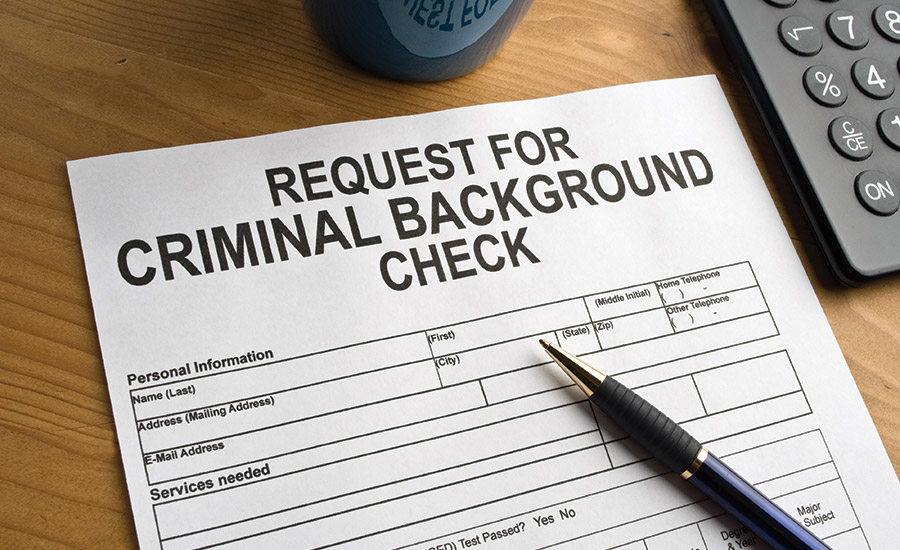
\includegraphics[width=.4\textwidth]{figs/criminal_record.jpg}
\end{center} \pause

\begin{itemize}
\tightlist
\item
  Does having a criminal record affect job prospects? \pause 
\item
  Experimental setting:\pause 

  \begin{itemize}
  \tightlist
  \item
    Randomly assign 4 hired ``confederates'' (2 White, 2 Black) to apply
    to different jobs in Milwaukee.\pause 
  \item
    Men were matched on physical appearance, self-presentation, age,
    etc.\pause 
  \item
    Confederates would alternate indicating they had a criminal
    record.\pause 
  \end{itemize}
\item
  Outcome of interest: receiving a callback from a potential employer.
\end{itemize}
\end{frame}

\begin{frame}{A tale of two applications}
\phantomsection\label{a-tale-of-two-applications}
\begin{center}
\begin{tabular}{ l | l  l }
     & Criminal Record  & Callback? \\ \hline
    Applicant 1 & Ex-felon & No \\ 
    Applicant 2 & No criminal record & Yes \\ 
\end{tabular}
\end{center}

\pause

\begin{itemize}
\tightlist
\item
  Did the first applicant not get a callback \textbf{because} they had a
  criminal record?
\end{itemize}
\end{frame}

\begin{frame}{Notation and Jargon}
\phantomsection\label{notation-and-jargon}
\begin{itemize}
\tightlist
\item
  \textbf{Unit} (indexed by \(i\)): job application for employer \pause 
\item
  \textbf{Treatment variable} \(T_i\): criminal record or not \pause 
\item
  \textbf{Treatment group} (treated units): applications with criminal
  record \pause
\item
  \textbf{Control group} (untreated units): applications without
  criminal record \pause
\item
  \textbf{Outcome variable} \(Y_i\): callback
\end{itemize}

\begin{center}  
\begin{tabular}{ l | l  l }
     & $T_i$ (ex-felon)  & $Y_i$ (callback) \\ \hline
    Ex-felon applicant & 1 & 0 \\ 
    Non-ex-felon applicant & 0  & 1 \\ 
\end{tabular}
\end{center}
\end{frame}

\begin{frame}{Causal effects and counterfactuals}
\phantomsection\label{causal-effects-and-counterfactuals}
\begin{itemize}
\tightlist
\item
  What does ``\(T_i\) causes \(Y_i\)'' mean? \(\rightsquigarrow\)
  \textbf{counterfactuals}, ``what if'' \pause
\item
  Would an employer treat criminal \& noncriminal applicants
  differently? \pause
\item
  Two \textbf{potential outcomes}: \pause

  \begin{itemize}
  \tightlist
  \item
    \(Y_i (1)\): would applicant \(i\) get a callback if applied as an
    ex-felon? \pause
  \item
    \(Y_i (0)\): would applicant \(i\) get a callback if applied not as
    an ex-felon? \pause
  \end{itemize}
\item
  \textbf{Causal effect}: \(Y_i (1)\) - \(Y_i (0)\) \pause

  \begin{itemize}
  \tightlist
  \item
    \(Y_i (1) - Y_i (0) = 0 \rightsquigarrow\) criminal record has no
    impact on callback \pause
  \item
    \(Y_i (1) - Y_i (0) = -1 \rightsquigarrow\) criminal record prevents
    callback \pause
  \item
    \(Y_i (1) - Y_i (0) = +1 \rightsquigarrow\) criminal record leads to
    callback
  \end{itemize}
\end{itemize}
\end{frame}

\begin{frame}{Potential Outcomes}
\phantomsection\label{potential-outcomes}
\begin{center}  
\begin{tabular}{ l | l  l  l  l}
     & $T_i$ (ex-felon)  & $Y_i$ (callback) & $Y_i (1)$ & $Y_i (0)$ \\ \hline
    Ex-felon applicant & 1 & 0 & 0 & ???\\ 
    Non-ex-felon applicant & 0  & 1 & ??? & 1 \\ 
\end{tabular}
\end{center}  \pause

\begin{itemize}
\tightlist
\item
  \textbf{Fundamental problem of causal inference}: \pause

  \begin{itemize}
  \tightlist
  \item
    We only observe one of the two potential outcomes. \pause
  \item
    Observe \(Y_i = Y_i (1)\) if \(T_i = 1\) or \(Y_i = Y_i (0)\) if
    \(T_i = 0\) \pause
  \end{itemize}
\item
  To infer causal effect, we need to infer the missing counterfactuals!
\end{itemize}
\end{frame}

\begin{frame}{How can we figure out counterfactuals?}
\phantomsection\label{how-can-we-figure-out-counterfactuals}
\begin{center}
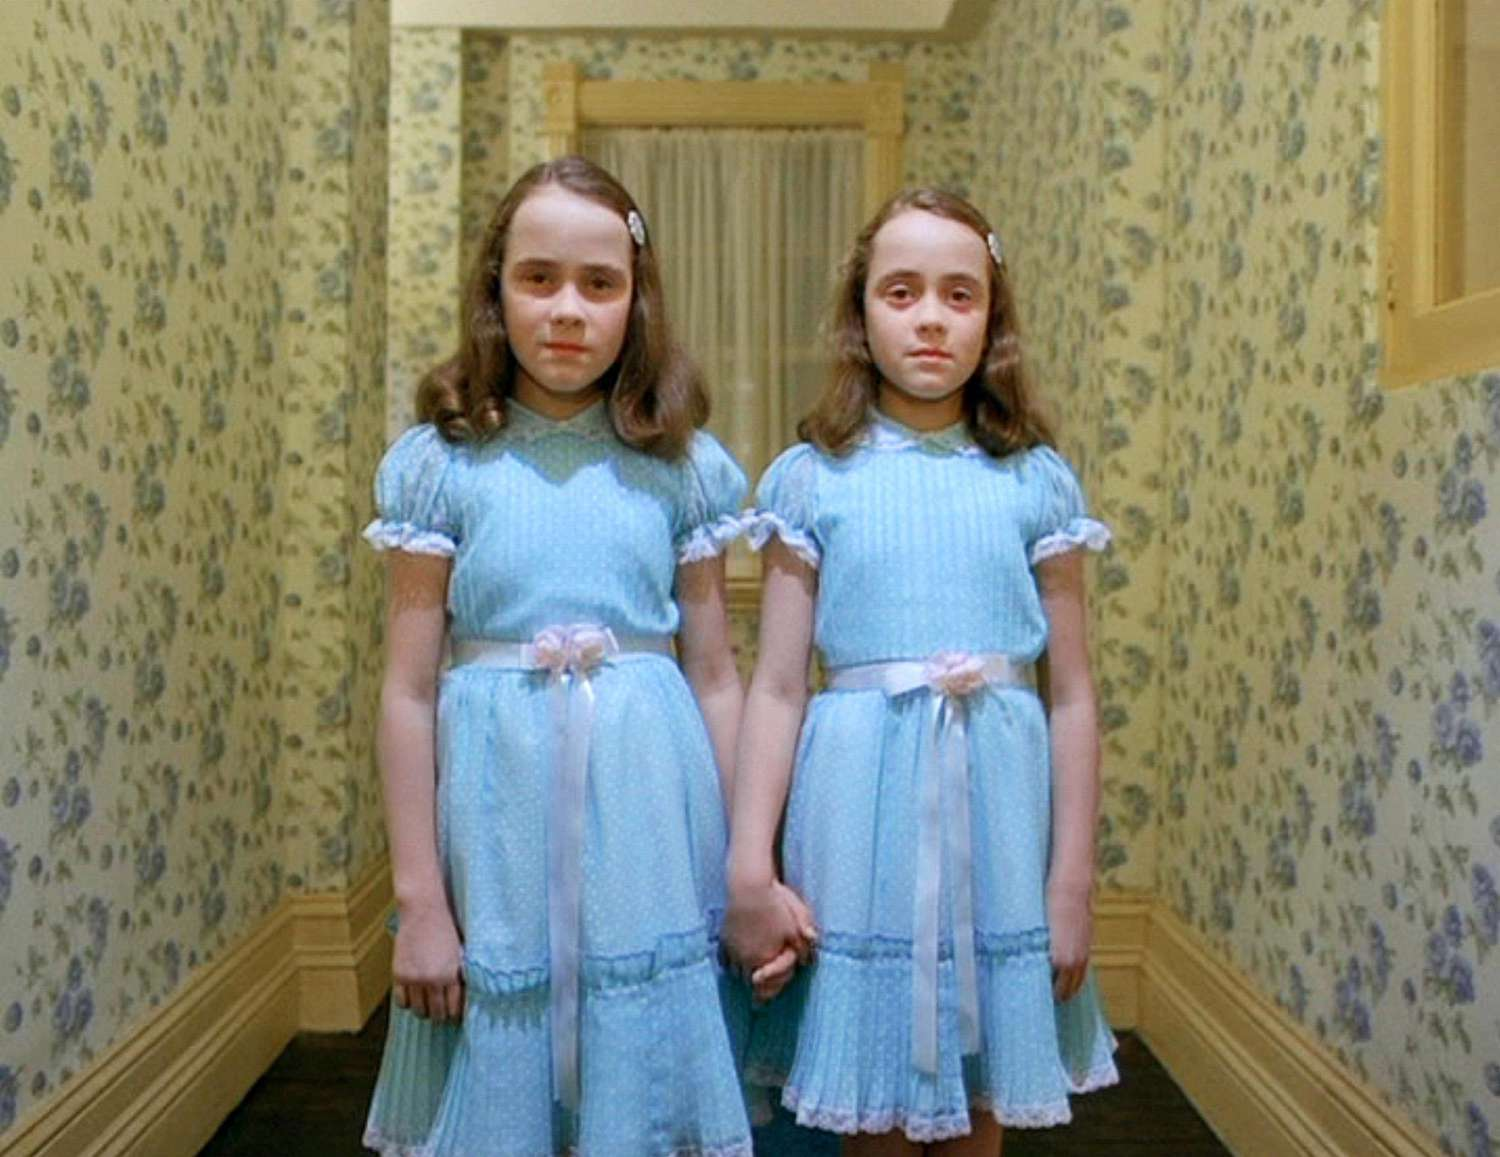
\includegraphics[width=.4\textwidth]{figs/shining.jpg}
\end{center}

\begin{itemize}
\tightlist
\item
  Find a similar unit! \(\rightsquigarrow\) \textbf{matching} (Mill's
  method of difference) \pause
\item
  Did applicant fail to get a job offer because of his criminal record?
  \pause

  \begin{itemize}
  \tightlist
  \item
    \(\rightsquigarrow\) find a non-ex-felon who is just like ex-felon
    applicant. \pause
  \end{itemize}
\item
  NJ increased the minimum wage. Causal effect on unemployment? \pause

  \begin{itemize}
  \tightlist
  \item
    \(\rightsquigarrow\) find a state similar to NJ that didn't increase
    minimum wage.
  \end{itemize}
\end{itemize}
\end{frame}

\begin{frame}{Imperfect matches}
\phantomsection\label{imperfect-matches}
\begin{columns}
  \begin{column}{0.4\textwidth}
    
\includegraphics[width=1\textwidth]{figs/twins.jpg}
  \end{column} \pause
  \begin{column}{0.6\textwidth}
  \begin{itemize}
  \item The problem: imperfect matches! \pause
  \item Say we match $i$ (treated) and $j$ (control) \pause
  \item \textbf{Selection Bias}: $Y_i (1) \neq Y_j (1)$  \pause
  \item Those who take treatment may be different that those who take control. \pause
  \item How can we correct for that?
  \end{itemize}
  \end{column}
\end{columns}
\end{frame}

\begin{frame}{Break time}
\phantomsection\label{break-time}
\begin{itemize}
\tightlist
\item
  Space here for a break in the action
\end{itemize}
\end{frame}

\begin{frame}{Changing minds on gay marriage}
\phantomsection\label{changing-minds-on-gay-marriage}
\begin{itemize}
\tightlist
\item
  Question: can we effectively persuade people to change their minds?
  \pause
\item
  Hugely important question for political campaigns, companies, etc.
  \pause
\item
  Psychological studies show it isn't easy. \pause
\item
  \textbf{Contact Hypothesis}: outgroup hostility diminished when people
  from different groups interact with one another. \pause
\item
  Today we'll explore this question the context of support for gay
  marriage and contact with a member of the LGBT community. \pause

  \begin{itemize}
  \tightlist
  \item
    \(Y_i =\) support for gay marriage (1) or not (0) \pause
  \item
    \(T_i =\) contact with member of the LGBT community (1) or not (0)
  \end{itemize}
\end{itemize}
\end{frame}

\begin{frame}{Causal effects and counterfactuals}
\phantomsection\label{causal-effects-and-counterfactuals-1}
\begin{itemize}
\tightlist
\item
  What does ``\(T_i\) causes \(Y_i\)'' mean? \(\rightsquigarrow\)
  \textbf{counterfactuals}, ``what if'' \pause
\item
  Would citizen \(i\) have supported gay marriage if they had contact
  with a member of the LGBT community? \pause
\item
  Two \textbf{potential outcomes}: \pause

  \begin{itemize}
  \tightlist
  \item
    \(Y_i(1)\): would \(i\) have supported gay marriage if they
    \textbf{had} contact with a member of the LGBT community? \pause
  \item
    \(Y_i(0)\): would \(i\) have supported gay marriage if they
    \textbf{didn't have} contact with a member of the LGBT community?
    \pause
  \end{itemize}
\item
  \textbf{Causal effect} for citizen \(i\): \(Y_i(1) - Y_i(0)\) \pause
\item
  \textbf{Fundamental problem of causal inference}: only one of the two
  potential outcomes is observable.
\end{itemize}
\end{frame}

\begin{frame}{Sigma notation}
\phantomsection\label{sigma-notation}
\begin{itemize}
\tightlist
\item
  We will often refer to the \textbf{sample size} (number of units) as
  \(n\). \pause
\item
  We often have \(n\) measurements of some variable:
  \((Y_1,Y_2,...,Y_n)\) \pause
\item
  We often want sums: how many in our sample support gay marriage?
  \pause
\end{itemize}

\[
  Y_1 + Y_2 + ... + Y_n 
  \]

\begin{itemize}
\tightlist
\item
  Notation is a bit clunky, so we often use the \textbf{Sigma notation}:
  \pause \[
    \sum_{i=1}^n Y_i = Y_1 + Y_2 + ... + Y_n
    \] \pause
\item
  \(\sum_{i=1}^n\) means sum each value from \(Y_1\) to \(Y_n\)
\end{itemize}
\end{frame}

\begin{frame}{Averages}
\phantomsection\label{averages}
\begin{itemize}
\item
  The \textbf{sample average} or \textbf{sample mean} is simply the sum
  of all values divided by the number of values. \pause
\item
  Sigma notation allows us to write this in a compact way: \pause
\end{itemize}

\[
  \bar{Y} = \frac{1}{n} \sum_{i=1}^n Y_i
  \]

\begin{itemize}
\tightlist
\item
  Suppose we surveyed 6 people and 3 supported gay marriage: \pause \[
    \bar{Y} = \frac{1}{6} (1 + 1 + 1 + 0 + 0 + 0) = 0.5
    \]
\end{itemize}
\end{frame}

\begin{frame}{Quantity of interest}
\phantomsection\label{quantity-of-interest}
\begin{itemize}
\tightlist
\item
  We want to estimate the average causal effects over all units:
  \vspace{-5pt} \pause
\end{itemize}

\[
  \text{Sample Average Treatment Effect (SATE) } = \frac{1}{n} \sum_{i=1}^n \left( Y_i(1) - Y_i(0) \right)
  \]

\begin{itemize}
\tightlist
\item
  Why can't we just calculate this quantity directly? \pause
\item
  What we can estimate instead: \vspace{-5pt} \pause
\end{itemize}

\[
  \text{Difference in means } = \bar{Y}_{treated} - \bar{Y}_{control}
  \]

\begin{itemize}
\tightlist
\item
  \(\bar{Y}_{treated}\): observed average outcome for treated group
\item
  \(\bar{Y}_{control}\): observed average outcome for control group
  \pause
\item
  When will the difference-in-means be a good estimate of the SATE?
\end{itemize}
\end{frame}

\begin{frame}{Randomized control trials (RCTs)}
\phantomsection\label{randomized-control-trials-rcts}
\begin{itemize}
\tightlist
\item
  \textbf{Randomize control trial}: each unit's treatment assignment is
  determined by chance \pause

  \begin{itemize}
  \tightlist
  \item
    e.g., flip a coin; draw read and blue chips from a hat; etc. \pause
  \end{itemize}
\item
  Randomization ensures \textbf{balance} between treatment and control
  group. \pause

  \begin{itemize}
  \tightlist
  \item
    Treatment and control group are identical \textbf{on average} \pause
  \item
    Similar on both observable and unobservable characteristics. \pause
  \end{itemize}
\item
  Control group \(\approx\) what would have happened to treatment group
  if they had taken control \pause

  \begin{itemize}
  \tightlist
  \item
    \(\bar{Y}_{control} \approx \frac{1}{n} \sum_{i=1}^n Y_i(0)\) \pause
  \item
    \(\bar{Y}_{treated} - \bar{Y}_{control} \approx\) SATE
  \end{itemize}
\end{itemize}
\end{frame}

\begin{frame}{Some potential problems with RCTs}
\phantomsection\label{some-potential-problems-with-rcts}
\begin{itemize}
\tightlist
\item
  \textbf{Placebo effects}: \pause

  \begin{itemize}
  \tightlist
  \item
    Respondents will be affected by any intervention, even if they
    shouldn't have any effect \pause
  \end{itemize}
\item
  \textbf{Hawthorne effects}: \pause

  \begin{itemize}
  \tightlist
  \item
    Respondents act differently just knowing that they are under study.
  \end{itemize}
\end{itemize}
\end{frame}

\begin{frame}{Balance checking}
\phantomsection\label{balance-checking}
\begin{itemize}
\tightlist
\item
  Can we determine if randomization ``worked''? \pause
\item
  If it did, we shouldn't see large differences between treatment and
  control group on \textbf{pretreatment variable} \pause

  \begin{itemize}
  \tightlist
  \item
    Pretreatment variable are those that are unaffected by treatment
    \pause
  \end{itemize}
\item
  We can check in the actual data for some pretreatment variable \(X\)
  \pause

  \begin{itemize}
  \tightlist
  \item
    \(\bar{X}_{treated}\): average value of variable for treated group
    \pause
  \item
    \(\bar{X}_{control}\): average value of variable for control group
    \pause
  \item
    Under randomization,
    \(\bar{X}_{treated} - \bar{X}_{control} \approx 0\)
  \end{itemize}
\end{itemize}
\end{frame}

\begin{frame}{Multiple treatments}
\phantomsection\label{multiple-treatments}
\begin{itemize}
\tightlist
\item
  Instead of 1 treatment, we might have multiple \textbf{treatment
  arms}: \pause

  \begin{itemize}
  \tightlist
  \item
    Control condition
  \item
    Treatment A
  \item
    Treatment B
  \item
    Treatment C, etc.
  \end{itemize}
\item
  In this case, we will look at multiple comparisons: \pause

  \begin{itemize}
  \tightlist
  \item
    \(\bar{Y}_{treated,A} - \bar{Y}_{control}\) \pause
  \item
    \(\bar{Y}_{treated,B} - \bar{Y}_{control}\) \pause
  \item
    \(\bar{Y}_{treated,A} - \bar{Y}_{treated,B}\) \pause
  \end{itemize}
\item
  If treatment arms are randomly assigned, these differences will be
  good estimators for each causal contrast.
\end{itemize}
\end{frame}

\end{document}
